% CVPR 2026 Paper Template; see https://github.com/cvpr-org/author-kit

\documentclass[10pt,twocolumn,letterpaper]{article}
\usepackage{makecell} 
\usepackage{graphicx}
\usepackage{multirow}
\usepackage{capt-of}   % 提供 \captionof
\usepackage{cuted}     % 提供 strip 环境
\usepackage[table]{xcolor}
\usepackage{tabularx,booktabs,array}
\usepackage{pifont}
\usepackage{subcaption}
\newcolumntype{Y}{>{\centering\arraybackslash}X}

%%%%%%%%% PAPER TYPE  - PLEASE UPDATE FOR FINAL VERSION
% \usepackage{cvpr}              % To produce the CAMERA-READY version
% \usepackage[review]{cvpr}      % To produce the REVIEW version
\usepackage[pagenumbers]{cvpr} % To force page numbers, e.g. for an arXiv version

% Import additional packages in the preamble file, before hyperref
\input{preamble}

% It is strongly recommended to use hyperref, especially for the review version.
% hyperref with option pagebackref eases the reviewers' job.
% Please disable hyperref *only* if you encounter grave issues, 
% e.g. with the file validation for the camera-ready version.
%
% If you comment hyperref and then uncomment it, you should delete *.aux before re-running LaTeX.
% (Or just hit 'q' on the first LaTeX run, let it finish, and you should be clear).
\definecolor{cvprblue}{rgb}{0.21,0.49,0.74}
\usepackage[pagebackref,breaklinks,colorlinks,allcolors=cvprblue]{hyperref}

%%%%%%%%% PAPER ID  - PLEASE UPDATE
% \def\paperID{***} % *** Enter the Paper ID here
\def\confName{CVPR}
\def\confYear{2026}

%%%%%%%%% TITLE - PLEASE UPDATE
\title{Scaling Up AI-Generated Image Detection with Generator-Aware Prototypes}

%%%%%%%%% AUTHORS - PLEASE UPDATE
\author{First Author\\
Institution1\\
Institution1 address\\
{\tt\small firstauthor@i1.org}
% For a paper whose authors are all at the same institution,
% omit the following lines up until the closing ``}''.
% Additional authors and addresses can be added with ``\and'',
% just like the second author.
% To save space, use either the email address or home page, not both
\and
Second Author\\
Institution2\\
First line of institution2 address\\
{\tt\small secondauthor@i2.org}
}

\begin{document}
\clearpage
\setcounter{page}{1}
\maketitlesupplementary

\appendix
We organize the supplementary in the following way:
\begin{itemize}
    \item Sec.~\ref{sec:pre-exp}: Detailed information of the introduced series of dataset build in previous section.
    \item Sec.~\ref{sec:benchmark}: Details of the 6 selected benchmarks. 
    \item Sec.~\ref{sec:baseline}: Introduction to the selected baselines.
    \item Sec.~\ref{sec:detailexp}: Detailed results of each test subsets.
    \item Sec.~\ref{sec:impledet}: Implementation details of the proposed method.
    \item Sec.~\ref{sec:additional_analysis}: Additional derivation and analysis.
    \item Sec.~\ref{sec:future}: Future perspectives towards reasoning-driven and embodied forensics.
\end{itemize}

\section{Settings of the toy dataset}
\label{sec:pre-exp}
In Sec.3, we introduce a series of datasets, comprising generated images from different numbers of generators. In this section we will give the constructing procedure of these datasets.

First, there are 8 generators in GenImage \cite{zhu2024genimage} dataset, in each generator subset, there are 1000 types of object mirroring the 1000 categories of ImageNet-1k \cite{imagenet}. We select generator subset composed of $n_g$ generators based on Tab.~\ref{tab:toydataset}. For each of the 1000 categories, we randomly sample $n_s$ images in each  generator subset. To pair real images, we randomly sample $n_s \times n_g$ images from the original ImageNet dataset. $n_s$ is determined via  $1000 \times n_s \times n_g=8000$.


For the last dataset, which consist of thousands of generators, we leverage Community-Forensics training dataset \cite{park2025commfor} for collecting, which is the same as our training dataset. we randomly sample 2 images from each generator in it, which consist of about 9000 generated images. Then we randomly sample 8,000 real images as before to construct the last dataset in the series.

\begin{table}[h]
    \centering
    \begin{tabular}{c|c|c}
    \toprule
     group & $n_g$ & Generator(s) \\ 
     \midrule
        1 &  1  & SDv1.4 \\
        2 &  2  & SDv1.4, BigGAN \\ 
        3 &  4 &  SDv1.4, BigGAN, VQDM, Glide \\
        4 &  8 & All GenImage \\
        \bottomrule
    \end{tabular}
    \caption{Generators used to build our datasets.}
    \label{tab:toydataset}
\end{table}

\section{Benchmarks}
\label{sec:benchmark}

We select 6 benchmarks to represent most existed generative models to evaluate the methods. Though some subsets have same or similar architecture, their training condition, sampling strategy and semantic content are not quite the same. Thus we preserve all subsets that have same name to simulate a variety of generated images.

\vspace{2mm}
\noindent
\textbf{Forensic Synthetic} \cite{wang2020cnn} contains a series of CNN-generated images, we select its GAN variants, including ProGAN \cite{karras2018progressive}, StyleGAN \cite{karras2019style}, StyleGAN2, CycleGAN \cite{CycleGAN}, StarGAN \cite{choi2018stargan}, GauGAN \cite{GauGAN}, BigGAN \cite{BigGAN}, and Deepfake \cite{Deepfake} for forgery face.

\vspace{2mm}
\noindent
\textbf{UFD} \cite{ojha2023towards} datasets expand the dataset above by introducing several early diffusion models and commercial APIs, including latent diffusion model \cite{rombach2022high}, Glide \cite{nichol2021glide} and Guided \cite{dhariwal2021diffusion} diffusion model.

\vspace{2mm}
\noindent
\textbf{GenImage} \cite{zhu2024genimage} provide a dataset trained on ImageNet-1k. It has 8 generative models in both GANs, Diffusion Models and Commercial APIs, including BigGAN \cite{BigGAN}, VQDM \cite{gu2022vector}, Stable Diffusions, Wukong \cite{Wukong}, ADM \cite{dhariwal2021diffusion} and Midjourney \cite{Midjourney}.

\vspace{2mm}
\noindent
\textbf{SynthBuster} \cite{synthbuster} provide an aligned dataset, where real images and generated images are all in PNG format, which makes it challenging for AIGI detectors that leverage format shortcut. Moreover the generated images are also from popular latent diffusions, including DALL-E, Stable Diffusions, Firefly\cite{AdobeFirefly} and Glide.

\vspace{2mm}
\noindent
\textbf{Chameleon} \cite{yan2024sanity} provides a sanity check for AI-generated image detection. They build a high quality dataset where generated images are source from internet and some unknown source. All images in this benchmark are said to be indistinguishable by human. Since all images are gather from the unknown source, there's only one subset in this benchmark.

\vspace{2mm}
\noindent
\textbf{Community Forensics Evaluation Set }\cite{park2025commfor} is build to evaluate the model's ability to generalize to unseen generators that trained in Community Forensics dataset. This evaluation dataset is also the most up-to-date dataset, containing generators like Deci Diffusion V2~\cite{DeciFoundationModels}, GALIP~\cite{tao2023galip}, KandinskyV2.2~\cite{kandinsky2023models}, Kvikontent~\cite{KvikontentMidjourney}, LCM-LoRA-SDv1.5, LCM-LoRA-SDXL, LCM-LoRA-SSD1B~\cite{luo2023lcmLora}, Stable Cascade~\cite{pernias2023stablecascade}, DF-GAN~\cite{tao2022df}, and HDiT~\cite{crowson2024scalable}.

Above all, we have 55 subsets for testing. Given the large scale of our training data, the training domain overlaps with several previously constructed datasets. Consequently, our evaluation comprises $29$ completely unseen generator subsets, the rest, even though seen in training set, still have a different generated condition. Sample images from the test set are shown in Fig. ~\ref{fig:datasets}.

\begin{figure*}[!t]
        \centering
        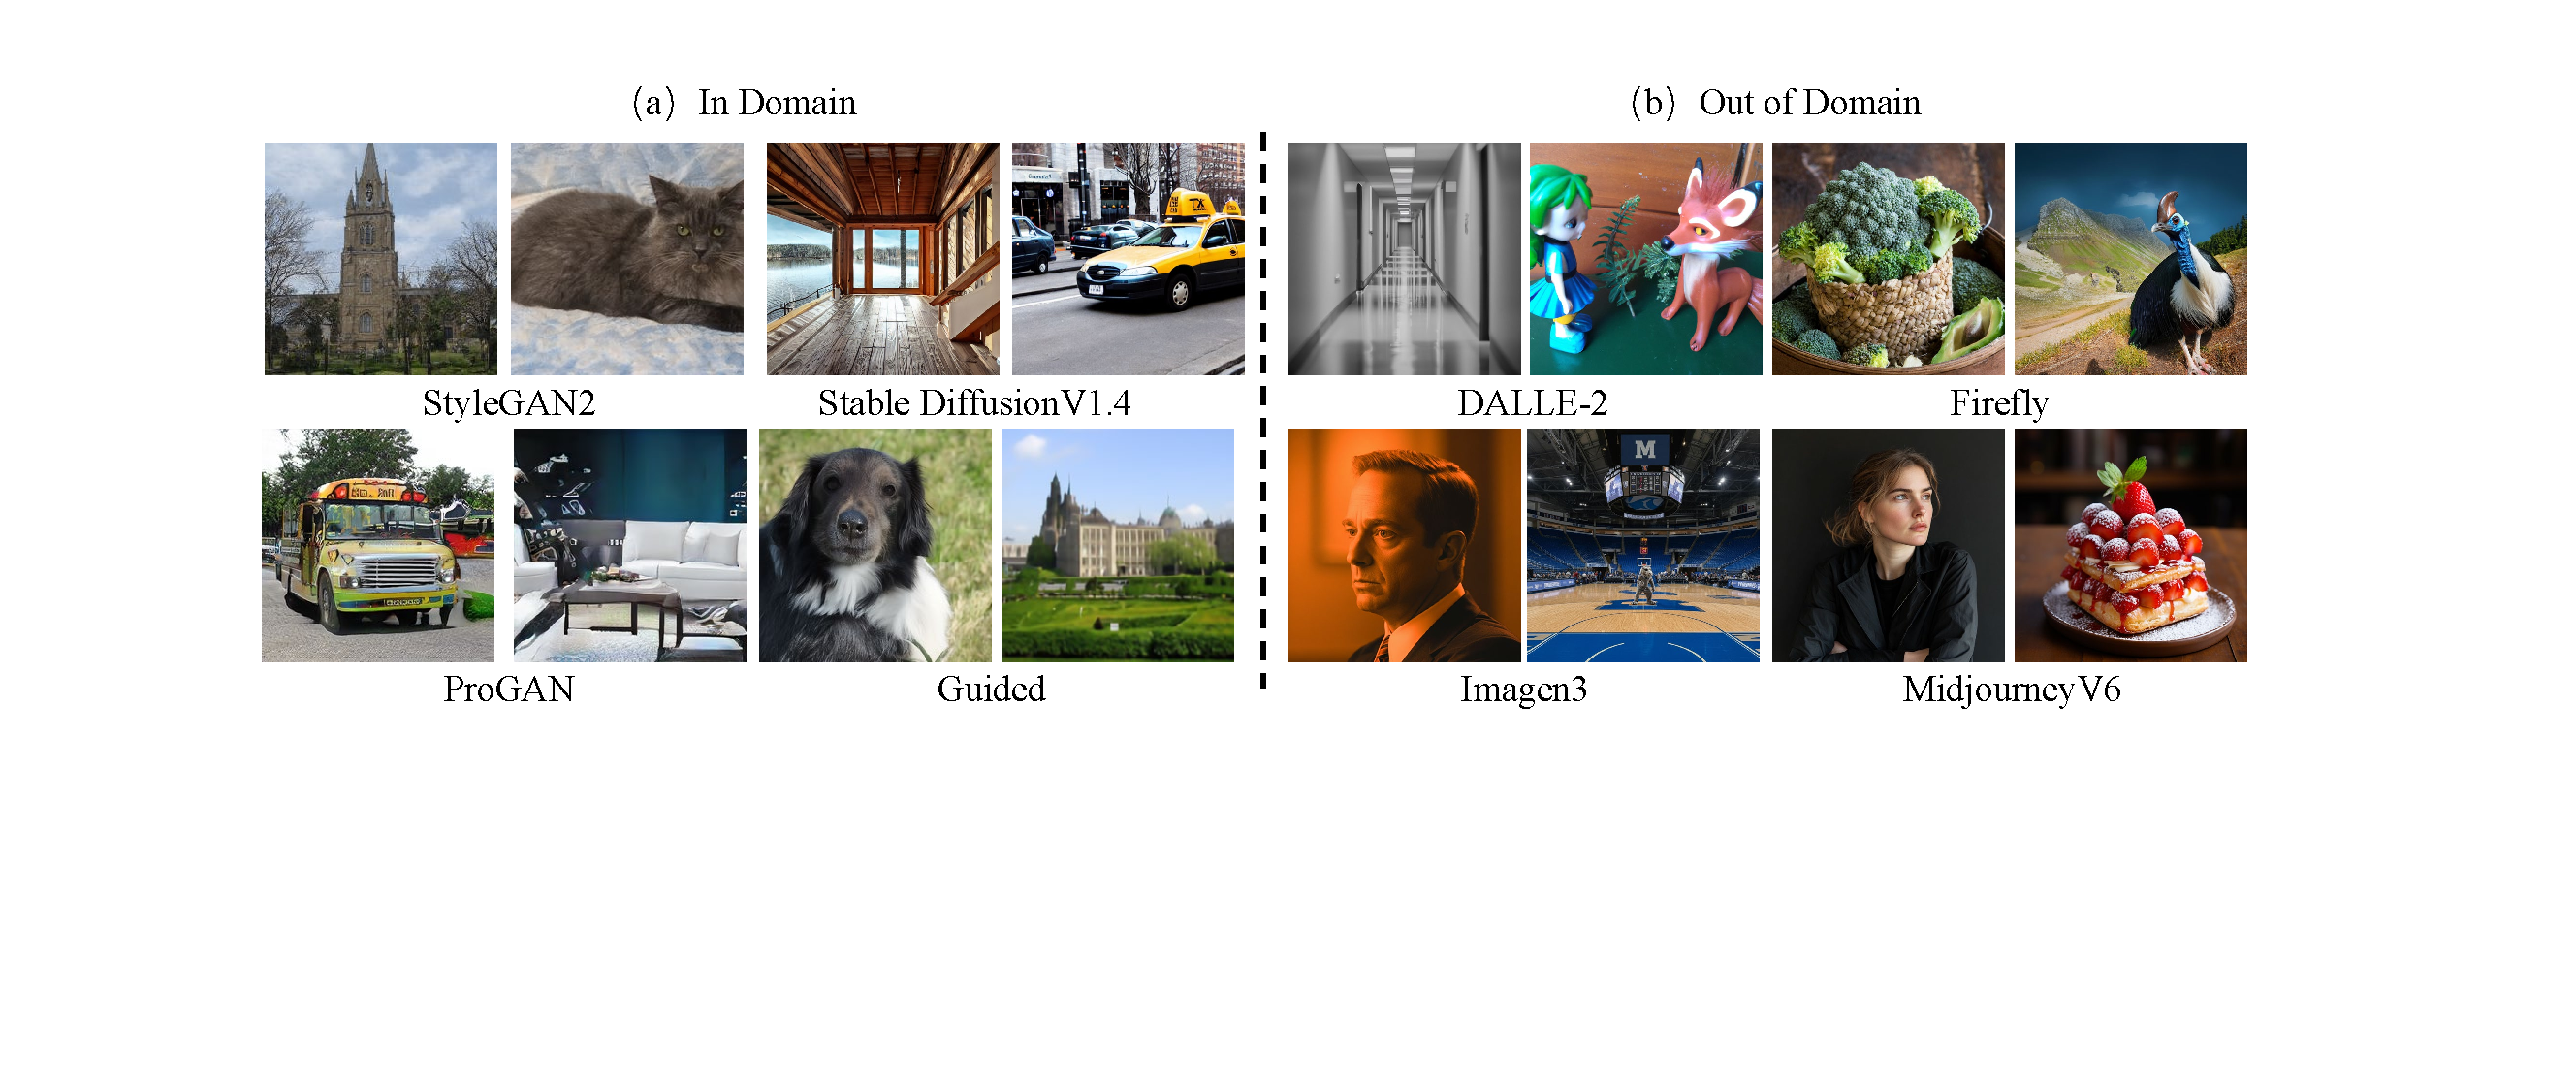
\includegraphics[width=\linewidth]{figs/datasets.pdf} 
        \caption{Examples of test subsets, we visualize some in-domain datasets with our training set along with some out-of-distribution sets. }
        \label{fig:datasets} 
\end{figure*}


\textbf{Metrics.} Following prior works \cite{wang2020cnn, ojha2023towards, tan2024rethinking}, we compute a threshold-free metric, mean average precision (AP), and a threshold-based metric, binary accuracy (Acc). When computing accuracy, the threshold was set to 0.5.

\section{Baselines}
\label{sec:baseline}
    In this section, we will give a brief introduction to the baselines for comparison.

\subsection{GAN-Generalized}
\textbf{CNNDetection} \cite{wang2020cnn} uses a ResNet-50 as a classifier with data augmentation to detect CNN-generated images. \textbf{NPR} \cite{tan2024rethinking} rethink up-sampling operation in most generative architecture and detect them via a interpolation pattern. \textbf{UniFD} \cite{ojha2023towards} leverage the image encoder of CLIP for feature extraction, it takes image embeddings for classification with simple KNN or linear layer. \textbf{SAFE}\cite{li2025improving} extracts high frequency band as artifact with various data augmentation to build a CNN classifier. \textbf{AIDE} uses a hybrid feature of both CLIP image embedding , high and low frequency patches via DCT scoring, and concatenate them for final decision. These baselines are all trained on GAN generated images provided by the training set of CNNDetection \cite{wang2020cnn}. 

\subsection{Diffusion-Generalized}
In the diffusion era \cite{rombach2022high}, more method aim to detect generated images with a more realistic diffusion generated images. \textbf{DRCT} \cite{chen2024drct} construct a diffusion reconstruct dataset and used it to train a classifier with classification objective and contrastive learning objective. We use its Conv-B variant trained on SDv2.1. \textbf{Co-SPY} \cite{cheng2025co} also uses a hybrid feature for classification, but a combination of CLIP embedding and VAE-reconstruct residual. \textbf{B-Free} \cite{Guillaro2024biasfree} proposed a paradigm that generated images should come from inpainting models rather than unconditional generators or T2Is to prevent semantic bias. It trained an end-to-end classifier with proposed dataset. 

\subsection{Scaling-Ups}
Scaling up detectors use a training dataset from a more diverse source. To solve the sanity check for AIGI detection, AIDE \cite{yan2024sanity} provide another checkpoint that trained a classifier with all images in GenImage, including both GANs and Diffusions. D3 \cite{yang2025d3} proposed a dual feature extraction branch, a original image and a patch-shuffled image to learn comprehensive traces, it uses a training dataset consist of GenImage and CNNDetection. Community Forensics construct a large dataset with thousands of generators and use it to train classifier with a standard ViT.

\section{Detailed results of experiments}
The following tables show detailed results for the selected 6 benchmarks. All baselines are evaluated with their provided checkpoints. Tab.~\ref{tab:Forensynths} shows results of ForenSynths, Tab.~\ref{tab:UFD} shows results of UFD, Tab.~\ref{tab:GenImage} shows results of GenImage, Tab.~\ref{tab:Synthbuster} shows results of SynthBuster, Tab.~\ref{tab:commfor1}
and Tab.~\ref{tab:commfor2} shows results of Community Forensics evaluation set.

\label{sec:detailexp}
\section{Implementation Details}
\label{sec:impledet}
To validate the reproducibility, we present our implementation details in this section.

\textbf{Network Design} The image encoder we use is CLIP:ViT-L with a patch size of $14 \times 14$. The MLP is composed of two hidden layer with dimensions $1024 \xrightarrow{} 128 \xrightarrow{} 1$. In the second stage, we discard the second layer to make the MLP $1024 \xrightarrow{} 128$, then we apply LoRA \cite{hu2022lora} in \texttt{q\_proj, k\_proj, v\_proj} of image encoder with LoRA parameter $r=16, \alpha=32, \text{dropout}=0.1$.

\textbf{Training} For image in training set, we apply RandomCrop to $224 \times 224$, and to those image whose resolution is smaller than this, we apply 0-padding to make it enough to crop. We automatically separate 5\%  samples of dataset to form a validation set. We use AdamW \cite{loshchilov2017decoupled} optimizer with a learning rate of $10^{-4}$ and a weight decay of $0.01$ in the two stages. In the first stage, training last for 20 epochs. In the second stage. we train until the validation accuracy reaches 99.9\% or do not improve for 3 epochs to prevent performance degradation.

\textbf{Testing} For images in testing sets, we apply CenterCrop to $224 \times 224$, which is the same as most baselines, except for \textbf{B-Free}, who uses a resolution of $504 \times 504$ and \textbf{Co-SPY} uses a $384 \times 384$, to best excel their performance, we did not modify their model but directly report their performance on original resolution.

\section{Additional Derivation and Analysis}
\label{sec:additional_analysis}

In this section, we provide supplementary materials to substantiate the claims made in the main text. Specifically, we present a rigorous mathematical derivation modeling the data heterogeneity in scaling-up settings (Sec.~\ref{sec:theory_derivation}) and offer qualitative visualizations of the attention maps to demonstrate how our method alters the encoder's focus (Sec.~\ref{sec:vis_attention}).

\subsection{Detailed Derivation of Theory}
\label{sec:theory_derivation}

Recall that in Sec.~3 of the main paper, we identified the ``Benefit then Conflict'' dilemma, attributing it to the severe data-level heterogeneity that arises when aggregating multiple generators. To theoretically quantify this phenomenon, we model the distribution of real and generated images and analyze the behavior of feature variance.

\textbf{Why GMM? How to calculate variance in GMM?}

We adopt the Gaussian Mixture Model (GMM) as a proxy for the real-world data distribution. This choice is motivated by the structure of commonly used datasets like ImageNet, which consist of distinct categories. Specifically, we model the image features within each category as a multivariate Gaussian distribution. While this is a simplified assumption, it remains theoretically robust and yields conclusions consistent with more complex scenarios. The total variance of the generated distribution is derived as follows:
\begin{equation}
    \Sigma_{gen}  = \mathbb{E}_G \left[ \text{Var}(X |G) \right] + \text{Var} _G\left[ \mathbb{E}(X|G)\right],
\end{equation}
For the $i$-th generator, its variance is computed by:
\begin{equation}
\begin{split}
    & Var(X|G=i)=\Sigma_{gen}^i \\
    & = \sum_{j=1}^{M}\pi_{i,j}\Sigma_{i,j} + \sum_{j=1}^{M}\pi_{i,j}(\mu_{i,j}-\mu_i)(\mu_{i,j}-\mu_i)^T
\end{split}
\end{equation}
Thus, the total variance can be expressed as:
\begin{equation}
\begin{split}
    \Sigma_{gen}&=\sum_{i}^{G}w_i\sum_{j}^{M}\pi_{i,j}\Sigma_{i,j} \\
     & + \sum_{i}^{G}w_i\sum_{j}^{M}\pi_{i,j}(\mu_{i,j}-\bar{\mu})(\mu_{i,j}-\bar{\mu})^T \\
     & + \sum_{i}^{G}w_i(\mu_{i}-\bar{\mu})(\mu_{i}-\bar{\mu})^T \\
     & = \underbrace{\mathbb{E}_M \left[ \text{Var}(X|G_i,M)|G_i\right]+\text{Var}_M\left[\mathbb{E}(X|G_i,M)|G_i \right]}_{\text{generator fitting variance}} \\
        & + \underbrace{\text{Var}_G \left[ \mathbb{E}(X|G)\right]}_{\text{cross generator variance}},
\end{split}
\end{equation}
where $\mu_i=\sum_{j}^{M}\pi_{i,j}\mu_{i,j}$, and $\bar{\mu}=\sum_{i}^{G}\mu_i$ denotes the mean within a generator and the global mean across the entire dataset, respectively.

\textbf{How do prototypes limit variance growth?}

Having established that variance increases with generator diversity, we now show how our prototype mapping strategy mitigates this issue. In prototype mapping, the feature embedding is reorganized into a linear combination of prototypes; this operation effectively sets an upper bound on the embedding's variance.

We have $ \tilde{f}=\sum w_i v_i$ where $w_i$ is the attention score and $v_i$ is a prototype vector. Let $F$ be the random variable of this reorganized embedding. Its variance is given by:
\begin{equation}
    Var(F)=\mathbb{E} \left[ || F-\mathbb{E}(F)||^2\right],
\end{equation}
where $Var(\cdot)$ here denotes its trace in the covariance matrix, i.e., $tr(\Sigma)$. To proceed, we introduce an independent identically distributed random variable $F'$ to reformulate this term as:
\begin{equation}
    \begin{aligned}
        Var(F)& =\frac{1}{2}\mathbb{E} \left[ ||F - F'||^2 \right] \\
        & = \frac{1}{2} \sum w_i w_j|| v_i-v_j||^2,
    \end{aligned}
\end{equation}
Assume $ D= \max_{v \in P}||v_i-v_j||$. Since all the prototypes are determined and fixed, this maximum distance is a constant. Due to the fact that $w_i, w_j \in [0,1]$ and $\sum w_i = 1$, this variance term can be bounded by:
\begin{equation}
    Var(F) \le \frac{1}{4}D^2.
\end{equation}
This derivation confirms that regardless of the number of source generators, the variance of the features mapped to the prototype space remains bounded by the geometry of the prototype set.

\subsection{Visualization of Attention Maps}
\label{sec:vis_attention}

To provide interpretability for our model's performance, we move beyond theoretical bounds to empirical visualization. We compare the attention maps from both the original CLIP image encoder and the encoder fine-tuned by our proposed GAPL. 

These attention maps represent the attention scores between the [CLS] token and all spatial patch tokens. The image encoder consists of 24 ViT blocks; in our visualization, we sample 8 blocks, with block indices ascending from left to right (shallow to deep). For visual clarity, bicubic interpolation is applied to the raw attention maps. As shown in Fig.~\ref{fig:attention1} and Fig.~\ref{fig:attention2}, the comparisons demonstrate two key findings: (1) Our encoder preserves rich semantic information in the shallow layers, maintaining the generalization capability of the pre-trained model; (2) In deeper layers, compared to the original CLIP, our model effectively leverages more patches to form a more comprehensive artifact pattern. Visually, this manifests as more pronounced and focused bright spots in the deeper layers, indicating that GAPL has successfully learned to attend to generator-specific traces.



\section{Future Perspectives}
\label{sec:future}

While our proposed GAPL framework achieves state-of-the-art performance by managing data heterogeneity through generator-aware prototypes, we recognize that the arms race between generation and detection is evolving. As generative models (e.g., Flux~\cite{blackforestlabs2024flux}, Midjourney v6~\cite{midjourneyv6}, Nano Banana Pro~\cite{banana}) increasingly mitigate low-level statistical artifacts, relying solely on texture or frequency cues may face diminishing returns. We envision that the next generation of AIGI detectors must integrate higher-level cognitive capabilities. Specifically, we identify three promising avenues where our scaling-up principles can intersect with broader AI domains:

\paragraph{From Artifact Detection to Visual Reasoning.}
Current forensic methods predominantly focus on signal-level anomalies. However, highly realistic AI-generated images often retain subtle \textit{semantic} or \textit{logical} inconsistencies (e.g., impossible shadows, mismatched reflections, or counting errors) that are invisible to standard classifiers. Future work should explore integrating \textbf{Visual Reasoning} frameworks~\cite{tanreason, ji2025mathsticks, ji2025visualtrans,song2025maniplvm} into the detection pipeline. By leveraging neuro-symbolic approaches or chain-of-thought reasoning, a detector could move beyond binary classification to provide interpretable evidence based on compositional logic, effectively identifying ``why'' an image violates reality even when pixel statistics appear perfect.

\paragraph{Incorporating Spatial Intelligence and Physical Constraints.}
A persistent weakness in current generative models is their frequent violation of 3D geometry and physical laws. While GAPL effectively learns 2D prototypes, it does not explicitly model the underlying 3D structure of the scene. Incorporating {spatial intelligence}~\cite{ji2025robobrain,team2025robobrain,wang2025crosspoint} could serve as a powerful orthogonal check. Models equipped with 3D-aware representations or spatial reasoning capabilities can detect geometric implausibilities—such as ``Escher-like'' structures or inconsistent depth cues—that purely 2D generative models fail to resolve. This aligns with our observation of ``Benefit then Conflict,'' suggesting that physical laws could serve as the ultimate invariant feature across diverse generators.

\paragraph{Trustworthy Perception in Embodied AI.}
Finally, the utility of AIGI detection extends beyond digital media forensics into the physical world. As we deploy autonomous agents, ensuring {trustworthy perception} is critical. Embodied agents operating in the real world must distinguish between authentic sensory inputs and potentially manipulated streams (e.g., adversarial projections or deepfakes in video feeds)~\cite{ji2025enhancing,bai2025alleviating}. Furthermore, robust detection models like GAPL can act as quality filters for {Embodied AI}~\cite{bai2025towards,lyu2025egoprompt,ji2025visualtrans,tan2025roboos}, particularly in Sim-to-Real pipelines where agents are trained on synthetic data. By rigorously curating high-fidelity synthetic data that adheres to physical realism, we can ensure that embodied agents develop robust representations that generalize better to physical reality.



\begin{table*}[t]
\centering
\renewcommand{\arraystretch}{1.1}
\resizebox{\textwidth}{!}{
\begin{tabular}{l cc cc cc cc cc cc cc cc cc}
\toprule
\multirow{2}{*}{\textbf{Method}} & \multicolumn{2}{c}{ProGAN} & \multicolumn{2}{c}{StyleGAN} & \multicolumn{2}{c}{StyleGAN2} & \multicolumn{2}{c}{StarGAN} & \multicolumn{2}{c}{GauGAN} & \multicolumn{2}{c}{CycleGAN} & \multicolumn{2}{c}{BigGAN} & \multicolumn{2}{c}{Deepfake} & \multicolumn{2}{c}{Mean} \\
\cmidrule(lr){2-3} \cmidrule(lr){4-5} \cmidrule(lr){6-7} \cmidrule(lr){8-9} \cmidrule(lr){10-11} \cmidrule(lr){12-13} \cmidrule(lr){14-15} \cmidrule(lr){16-17} \cmidrule(lr){18-19}
& Acc & AP &  Acc & AP & Acc & AP& Acc & AP&  Acc & AP & Acc & AP& Acc & AP & Acc & AP & Acc & AP \\
\midrule
CNNDet \cite{wang2020cnn} & 100.0 & 100.0 & 74.3 & 98.4 & 76.3 & 92.1 & 81.1 & 95.3 & 80.1 & 98.0 & 81.1 & 96.4 & 59.5 & 88.2 & 51.0 & 66.1 & 75.3 $\pm$ 13.9 & 91.8 $\pm$ 10.3 \\ 
NPR \cite{tan2024rethinking}  & 99.8 & 99.9 & 97.3 & 99.9 & 99.5 & 100 & 99.7 & 100 & 79.1 & 80.2 & 94.5 & 97.6 & 83.6 & 84.7 & 73.7 & 72.5 & 90.1 $\pm$ 9.9 & 91.8 $\pm$ 10.3 \\
UniFD \cite{ojha2023towards} &  99.8 & 100.0 & 85.4 & 97.5 & 74.5 & 97.6 & 96.0 & 99.5 & 99.4 & 100.0 & 98.3 & 99.8 & 94.7 & 99.2 & 67.5 & 80.3 & 89.4 $\pm$  11.6 & 96.7 $\pm$  6.3 \\
SAFE \cite{li2025improving} & 99.8 & 100.0 & 97.6 & 99.8 & 98.7 & 100.0 & 99.8 & 100.0 & 92.2 & 96.9 & 99.1 & 99.8 & 89.5 & 95.1 & 93.2 & 97.2 & 96.2  $\pm$ 3.7 & 98.6 $\pm$ 1.8 \\
AIDE \cite{yan2024sanity} & 96.3 & 99.8 & 97.2 & 99.7 & 98.1 & 99.8 & 98.4 & 99.9 & 76.9 & 96.0 & 95.6 & 99.4 & 78.3 & 96.7 & 54.2 & 68.7 & 86.8 $\pm$  14.9 & 95.0 $\pm$ 10.0 \\
DRCT \cite{chen2024drct} &  50.2 & 50.2 & 49.1 & 49.1 & 49.3 & 45.3 & 38.3 & 38.7 & 49.9 & 43.2 & 49.3 & 44.6 & 49.7 & 47.8 & 64.7 & 78.4 & 50.1 $\pm$ 6.7 & 49.6 $\pm$ 11.4 \\
Co-SPY \cite{cheng2025co} & 74.7 & 78.1 & 63.7 & 69.8 & 59.7 & 62.9 & 62.1 & 94.3 & 69.6 & 83.4 & 58.5 & 55.8 & 71.6 & 83.9 & 64.9 & 78.7 & 65.6 $\pm$ 5.4 & 75.9 $\pm$ 11.6 \\
B-Free \cite{Guillaro2024biasfree} & 95.6 & 99.3 & 74.8 & 93.6 & 71.1 & 89.4 & 81.1 & 93.5 & 96.0 & 99.8 & 65.4 & 90.5 & 91.5 & 98.9 & 73.7 & 89.2 & 81.2 $\pm$  11.1 & 94.3 $\pm$ 4.2  \\ 
AIDE$\dagger$ \cite{yan2024sanity} & 92.7 & 98.8 & 88.6 & 95.1 & 93.6 & 98.6 & 88.0 & 99.0 & 87.7 & 98.9 & 92.0 & 98.9 & 84.9 & 97.7 & 54.8 & 63.2 & 85.3 $\pm$  11.8 & 93.8 $\pm$ 11.6 \\
D3 \cite{yang2025d3} & 99.8 & 100.0 & 93.5 & 99.1 & 95.8 & 99.5 & 93.5 & 98.7 & 98.7 & 100.0 & 95.9 & 99.5 & 99.6 & 100.0 & 67.5 & 87.0 & 93.0 $\pm$ 9.9 & 98.0 $\pm$ 4.2 \\
CommForen \cite{park2025commfor} & 92.8 & 99.8 & 93.1 & 99.3 & 92.7 & 99.5 &  98.8 & 99.9 & 98.8 & 99.9 & 95.5 & 99.8 & 99.6 & 100.0 & 66.8 & 88.9 & 92.2 $\pm$ 10.0 & 98.2 $\pm$ 3.6 \\
\rowcolor{cvprblue!20} 
GAPL(Ours) & 99.9 & 100.0 & 98.1 & 100.0 & 99.5 & 100.0 & 97.0 & 99.9 & 99.6 & 100.0 & 98.2 & 99.9 & 98.6 & 100.0 & 88.2 & 96.8 & 97.2 $\pm$ 3.6 & 99.5 $\pm$ 1.1 \\
\bottomrule
\end{tabular}
}
\caption{Detaild results on the benchmark ForenSynth \cite{wang2020cnn}. we only select its GAN variant. $\text{AIDE}^{\dagger}$ denotes its scaling up checkpoint trained on 8 generators.}
\label{tab:Forensynths}
\end{table*}


\begin{table*}[!t]
\centering
\renewcommand{\arraystretch}{1.1}
\resizebox{\textwidth}{!}{
\begin{tabular}{l cc cc cc cc cc cc cc cc cc}
\toprule
\multirow{2}{*}{\textbf{Method}} & \multicolumn{2}{c}{DALL-E} & \multicolumn{2}{c}{Glide-50-27} & \multicolumn{2}{c}{Glide-100-10} & \multicolumn{2}{c}{Glide-100-27} & \multicolumn{2}{c}{Guided} & \multicolumn{2}{c}{LDM-100} & \multicolumn{2}{c}{LDM-200} & \multicolumn{2}{c}{LDM-200-cfg} & \multicolumn{2}{c}{Mean} \\
\cmidrule(lr){2-3} \cmidrule(lr){4-5} \cmidrule(lr){6-7} \cmidrule(lr){8-9} \cmidrule(lr){10-11} \cmidrule(lr){12-13} \cmidrule(lr){14-15} \cmidrule(lr){16-17} \cmidrule(lr){18-19}
& Acc & AP &  Acc & AP & Acc & AP& Acc & AP&  Acc & AP & Acc & AP& Acc & AP & Acc & AP & Acc & AP \\
\midrule
CNNDet \cite{wang2020cnn} & 52.9 & 68.4 & 55.7 & 78.0 & 54.3 & 74.3 & 53.3 & 73.7 & 52.8 & 68.1 & 52.0 & 68.7 & 51.5 & 68.2 & 52.2 & 69.6 & 53.1 $\pm$ 1.3 & 71.1 $\pm$3.5  \\ 
NPR \cite{tan2024rethinking}  & 90.3 & 97.4 & 97.2 & 99.2 & 97.6 & 99.2 & 96.9 & 99.1 & 87.1 & 92.6 & 97.4 & 99.1 & 97.6 & 99.2 & 97.4 & 99.0 & 95.2 $\pm$ 3.8 & 98.1 $\pm$ 2.2 \\
UniFD \cite{ojha2023towards} & 87.5 & 97.7 & 79.2 & 96.0 & 78.0 & 95.5 & 78.7 & 95.8 & 70.0 & 88.3 & 95.2 & 99.3 & 94.5 & 99.4 & 74.2 & 93.2 & 82.2 $\pm$ 8.7 & 95.7$\pm$ 3.4 \\
SAFE \cite{li2025improving} & 97.5 & 99.7 & 96.6 & 99.2 & 97.3 & 99.4 & 95.8 & 98.9 & 82.4 & 95.8 & 98.8 & 100.0 & 98.8 & 100.0 & 98.7 & 99.9 & 95.7 $\pm$5.1 & 99.1 $\pm$ 1.3 \\
AIDE \cite{yan2024sanity} & 89.7 & 99.6 & 89.9 & 99.8 & 89.8 & 99.6 & 89.9 & 99.8 & 94.2 & 98.9 & 90.1 & 99.9 & 90.1 & 99.9 & 90.1 & 99.9 & 90.5 $\pm$1.4 & 99.7 $\pm$ 0.3 \\
DRCT \cite{chen2024drct} & 55.6 & 57.8 & 56.2 & 62.6 & 61.0 & 70.4 & 56.2 & 62.7 & 62.6 & 89.3 & 88.8 & 96.6 & 88.9 & 96.7 & 90.3 & 97.5 & 70.0 $\pm$ 15.2 & 79.2 $\pm$16.3  \\
Co-SPY \cite{cheng2025co} & 81.8 & 87.2 & 69.0 & 74.6 & 76.7 & 81.7 & 73.5 & 78.2 & 62.7 & 87.4 & 82.7 & 86.9 & 83.1 & 87.5 & 85.2 & 91.0 & 76.8 $\pm$7.4 & 84.3 $\pm$5.2 \\
B-Free \cite{Guillaro2024biasfree} & 93.2 & 97.9 & 78.6 & 90.2 & 81.8 & 91.9 & 77.9 & 89.4 & 74.6 & 93.6 & 97.2 & 99.9 & 97.1 & 99.8 & 96.9 & 99.8 & 87.1 $\pm$9.2 & 95.3 $\pm$ 4.2 \\ 
AIDE$^\dagger$ \cite{yan2024sanity} & 98.7 & 99.9 & 99.0 & 100.0 & 99.1 & 100.0 & 99.0 & 100.0 & 95.5 & 99.9 & 99.1 & 100.0 & 99.1 & 100.0 & 99.1 & 100.0 & 98.6 $\pm$ 1.1 & 100.0 $\pm$ 0 \\
D3 \cite{yang2025d3} & 94.0 & 98.7 & 95.8 & 99.3 & 95.8 & 99.4 & 95.7 & 99.5 & 95.9 & 99.6 & 96.1 & 99.7 & 95.8 & 99.7 & 89.3 & 96.5 & 94.8 $\pm$ 2.2& 99.0 $\pm$ 1.0 \\
CommForen \cite{park2025commfor} & 98.4 & 99.9 & 97.1 & 99.6 & 98.2 & 99.8 & 96.8 & 99.6 & 66.1 & 76.6 & 98.5 & 99.9 & 98.7 & 99.9 & 98.5 & 99.9 & 94.0 $\pm$ 10.5 & 96.9 7.6 \\
\rowcolor{cvprblue!20} 
GAPL(Ours) & 97.8 & 100.0 & 97.7 & 99.9 & 97.8 & 100 & 97.7 & 100.0 &  93.4 & 98.6 &  97.8 & 100.0 & 97.9 & 100.0 & 97.9 & 100 & 97.2 $\pm$ 1.5  & 99.8 $\pm$ 0.5 \\
\bottomrule
\end{tabular}
}
\caption{Detaild results on the benchmark UFD. We refer this set to the diffusion part that \cite{ojha2023towards} added. }
\label{tab:UFD}
\end{table*}


\begin{table*}[!t]
\centering
\renewcommand{\arraystretch}{1.1}
\resizebox{\textwidth}{!}{
\begin{tabular}{l cc cc cc cc cc cc cc cc cc}
\toprule
\multirow{2}{*}{\textbf{Method}} & \multicolumn{2}{c}{VQDM} & \multicolumn{2}{c}{SDv1.4} & \multicolumn{2}{c}{BigGAN} & \multicolumn{2}{c}{Wukong} & \multicolumn{2}{c}{SDv1.5} & \multicolumn{2}{c}{Glide} & \multicolumn{2}{c}{Midjourney} & \multicolumn{2}{c}{ADM} & \multicolumn{2}{c}{Mean} \\
\cmidrule(lr){2-3} \cmidrule(lr){4-5} \cmidrule(lr){6-7} \cmidrule(lr){8-9} \cmidrule(lr){10-11} \cmidrule(lr){12-13} \cmidrule(lr){14-15} \cmidrule(lr){16-17} \cmidrule(lr){18-19}
& Acc & AP &  Acc & AP & Acc & AP& Acc & AP&  Acc & AP & Acc & AP& Acc & AP & Acc & AP & Acc & AP \\
\midrule
CNNDet \cite{wang2020cnn} & 52.1 & 68.8 & 50.5 & 59.8 & 51.2 & 78.6 & 50.8 & 59.3 & 50.7 & 60.6 & 52.3 & 67.6 & 51.3 & 64.7 & 51.5 & 65.6 & 51.3 $\pm$  0.6 & 65.6 $\pm$ 5.9  \\ 
NPR \cite{tan2024rethinking}  & 89.6 & 94.1 & 92.1 & 95.0 & 70.1 & 80.3 & 88.0 & 93.0 & 91.7 & 95.4 & 93.2 & 96.5 & 79.7 & 86.5 & 85.7 & 91.7 & 86.2 $\pm$ 7.3 & 91.6 $\pm$ 
 5.1 \\
UniFD \cite{ojha2023towards} & 84.0 & 96.3 & 64.1 & 87.4 & 89.8 & 98.5 & 71.8 & 91.2 & 64.4 & 86.0 & 61.6 & 84.6 & 57.2 & 75.5 & 67.1 & 86.8 & 70.0 $\pm$ 10.6 & 88.3 $\pm$  6.7 \\
SAFE \cite{li2025improving} & 96.1 & 99.6 & 99.4 & 100.0 & 97.6 & 99.8 & 98.1 & 99.8 & 98.8 & 99.9 & 97.2 & 99.6 & 95.5 & 99.5 & 81.5 & 96.4 & 95.5 $\pm$ 5.4 & 99.3 $\pm$ 1.1\\
AIDE \cite{yan2024sanity} & 98.4 & 99.9 & 98.3 & 99.9 & 98.9 & 99.9 & 97.3 & 99.8 & 98.1 & 99.8 & 98.6 & 99.9 & 86.4 & 96.6 & 96.8 & 99.5 & 96.6 $\pm$ 3.9 & 99.4 $\pm$ 1.1  \\
DRCT \cite{chen2024drct} & 61.3 & 85.4 & 97.9 & 99.8 & 52.3 & 86.3 & 95.9 & 99.6 & 97.9 & 99.8 & 60.1 & 91.2 & 98.2 & 99.9 & 60.0 & 90.2 & 78.0 $\pm$ 20.0 & 94.0 $\pm$  6.0 \\
Co-SPY \cite{cheng2025co} & 72.2 & 93.9 & 93.1 & 99.2 & 64.7 & 90.8 & 91.2 & 98.8 & 93.0 & 99.0 & 81.4 & 96.5 & 70.0 & 91.0 & 58.8 & 84.3 & 78.0 $\pm$  12.7 & 94.2 $\pm$  4.9 \\
B-Free \cite{Guillaro2024biasfree} & 88.2 & 98.3 & 99.4 & 100.0 & 76.5 & 96.8 & 99.4 & 100.0 & 99.3 & 100.0 & 69.7 & 93.8 & 94.1 & 99.3 & 72.5 & 93.7 & 87.4 $\pm$ 11.9 & 97.7 $\pm$  2.5 \\ 
AIDE$^\dagger$ \cite{yan2024sanity} & 99.9 & 100.0 & 99.8 & 100.0 & 99.9 & 100.0 & 99.6 & 100.0 & 99.8 & 100.0 & 99.8 & 100.0 & 99.0 & 100.0 & 99.5 & 100.0 & 99.7 $\pm$ 
 0.2 & 100.0$\pm$  0\\
D3 \cite{yang2025d3} & 98.3 & 99.9 & 98.1 & 99.8 & 97.1 & 99.7 & 97.7 & 99.8 & 97.7 & 99.8 & 98.3 & 99.8 & 79.7 & 95.8 & 96.8 & 99.6 & 95.5 $\pm$  6.0  & 99.3 $\pm$ 1.3  \\
CommForen \cite{park2025commfor} & 90.9 & 99.7 & 90.6 & 99.2 & 71.5 & 81.6 & 91.0 & 99.1 & 90.5 & 99.2 & 89.4 & 98.4 & 77.5 & 86.8 & 72.9 & 83.5 & 84.3 $\pm$ 8.1 & 93.4 $\pm$ 7.5\\
\rowcolor{cvprblue!20} 
GAPL(Ours) & 98.2 & 100 & 98.2 & 100 & 97.9 & 99.8 &  98.1 & 99.9 & 98.0 & 99.9 & 98.1 & 99.9 & 90.3 & 97.6 & 95.0 & 99.2 & 96.7$\pm$ 2.6 & 99.6 $\pm$ 0.7 \\
\bottomrule
\end{tabular}
}
\caption{Detaild results on the benchmark GenImage.}
\label{tab:GenImage}
\end{table*}

\clearpage

\begin{table*}[!t]
\centering
\renewcommand{\arraystretch}{1.1}
\resizebox{\textwidth}{!}{
\begin{tabular}{l c| cc cc cc cc cc cc cc cc cc cc}
\toprule
\multirow{2}{*}{\textbf{Method}} & \multicolumn{1}{c|}{Real} & \multicolumn{2}{c}{DALLE-2} & \multicolumn{2}{c}{Firefly} & \multicolumn{2}{c}{SDv1.4} & \multicolumn{2}{c}{SDXL} & \multicolumn{2}{c}{DALLE-3} & \multicolumn{2}{c}{Glide} & \multicolumn{2}{c}{MJ-v5} &\multicolumn{2}{c}{SDv1.3} & \multicolumn{2}{c}{SDv2} & \multicolumn{2}{c}{Mean} \\

\cmidrule(lr){2-2} \cmidrule(lr){3-4} \cmidrule(lr){5-6} \cmidrule(lr){7-8} \cmidrule(lr){9-10} \cmidrule(lr){11-12} \cmidrule(lr){13-14} \cmidrule(lr){15-16} \cmidrule(lr){17-18} \cmidrule(lr){19-20} \cmidrule(lr){21-22}
& Acc & Acc & AP & Acc & AP & Acc & AP& Acc & AP& Acc & AP & Acc & AP& Acc & AP & Acc & AP & Acc & AP & Acc & AP \\
\midrule
CNNDet \cite{wang2020cnn} & 96.5 & 7.0 & 64.8 & 14.4 & 74.9 & 1.5 & 49.9 & 5.2 & 59.0 & 0.1 & 36.2 & 1.8 & 46.9 & 1.2 & 44.8 & 1.3 & 49.3 & 4.8 & 96.5 & 50.3 $\pm$ 2.1 & 54.0 $\pm$ 17.9\\ 
NPR \cite{tan2024rethinking}  & 5.6 & 98.4 & 49.6 & 5.2 & 33.3 & 94.3 & 50.6 & 100 & 54.7 & 15.5 & 31.0 & 91.6 & 50.8 & 80.5 & 46.1 & 94.3 & 50.0 & 70.4 & 42.7 & 38.9 $\pm$17.1  & 45.4$\pm$7.7 \\
UniFD \cite{ojha2023towards} & 93.5 & 77.0 & 95.2 & 86.0 & 97.4 & 45.6 & 85.3 & 41.4 & 83.5 & 0.7 & 41.2 & 11.5 & 63.5 & 10.4 & 61.0 &44.8 & 85.3 &58.6 & 89.9 & 67.6 $\pm$14.0 & 78.0 $\pm$ 17.6 \\
SAFE \cite{li2025improving} & 15.5 & 92.0 & 42.2 & 4.3 & 31.0 & 91.8 & 55.9 & 87.4 & 37.1 & 44.5 & 34.7 & 58.1 & 36.0 & 97.0 & 54.8 & 91.0 & 53.9 & 99.5 & 56.5 & 44.7$\pm$15.1 & 44.7 $\pm$ 9.8\\
AIDE \cite{yan2024sanity} & 66.7 & 45.7 & 57.0 & 0.0 & 30.8 & 95.1 & 94.8 & 98.2 & 94.3 & 2.8 & 35.9 & 96.7 & 95.7 & 75.3 & 80.3 & 95.8 & 95.3 & 95.6 & 93.3 & 67.0 $\pm$ 19.3 & 75.3 $\pm$25.3  \\
DRCT \cite{chen2024drct} & 96.1 & 4.1 & 53.6 & 11.4 & 60.7 & 88.2 & 97.9 & 89.6 & 98.2 & 35.6 & 80.8 &  14.1 & 72.9 & 99.4 & 99.9 & 89.6 & 98.2 & 99.9 & 100.0 & 77.6 $\pm$ 19.6 & 84.7$\pm$ 17.3 \\
Co-SPY \cite{cheng2025co} & 97.6 & 48.5 & 90.8 & 43.6 & 87.5 & 74.7 & 96.4 & 44.1 & 87.9 & 73.7 & 96.5 & 80.6 & 97.8 & 35.2 & 85.0 & 74.5 & 96.7 & 40.0 & 85.4 & 77.4 $\pm$ 8.6  & 91.6 $\pm$ 5.0 \\
B-Free \cite{Guillaro2024biasfree} & 98.5 & 88.5 & 98.9 & 99.2 & 99.9 & 99.8 & 99.9 & 100.0 & 100.0 & 93.1 & 99.4 & 42.7 & 91.8 & 98.9 & 99.9 & 100.0 & 100.0 & 99.5 & 99.9 & 94.9$\pm$ 8.8  & 98.9 $\pm$ 2.5 \\ 
AIDE$^\dagger$ \cite{yan2024sanity} & 32.8 & 27.3 & 35.8 & 0.3 & 31.5 & 99.0 & 64.4 & 98.6 & 64.8 & 34.8 & 43.4 & 97.1 & 66.8 & 98.6 & 75.0 & 99.7 & 65.8 & 96.7 & 57.0 & 52.7 $\pm$ 18.8& 56.0 $\pm$ 14.5 \\
D3 \cite{yang2025d3} & 82.0 & 87.7 & 92.6 & 92.0 & 95.3 & 96.5 & 97.9 & 89.4 & 93.6 & 28.6 & 61.3 & 90.6 & 95.3 & 62.6 &81.2 & 96.4 & 97.7 & 82.6 & 90.8 & 81.3 $\pm$ 10.4 & 89.5  $\pm$ 11.0 \\
CommForen \cite{park2025commfor} & 84.6 & 83.9 & 91.6 & 93.1 & 96.6 & 94.7 & 97.4 & 98.5 & 98.3 & 76.1 & 88.4 & 90.0 & 96.0 & 80.6 & 91.4 & 95.7 & 97.7 & 92.9 & 95.3 & 87.1 $\pm$3.6 & 94.8 $\pm$ 3.3 \\
\rowcolor{cvprblue!20} 
GAPL(Ours) & 90.0 & 94.0 & 97.5 & 94.3 & 98.2 & 98.1 & 99.3 & 99.8 & 99.8 & 60.1 & 85.3 & 97.6 & 99.2 & 92.0 & 97.4 & 98.2 & 99.3 & 96.4 & 98.7 & 91.1 $\pm$ 5.8 & 97.2 $\pm$4.3 \\
\bottomrule
\end{tabular}
}
\caption{Detailed results on the benchmark SynthBuster \cite{synthbuster}. In this benchmark, all generated images are pair with exactly the same real images. Thus we report the real images accuracy and each generator's fake accuracy independently. We pair the metrics of real and each generators to get the final mean metrics .}
\label{tab:Synthbuster}
\end{table*}

\begin{table*}[!t]
\centering
\renewcommand{\arraystretch}{1.1}
\resizebox{\textwidth}{!}{
\begin{tabular}{l cc cc cc cc cc cc cc cc cc cc cc}
\toprule
\multirow{2}{*}{\textbf{Method}} & \multicolumn{2}{c}{DFGAN} & \multicolumn{2}{c}{MJv6} & \multicolumn{2}{c}{Kandinsky} & \multicolumn{2}{c}{SDcas.} & \multicolumn{2}{c}{MJv5} & \multicolumn{2}{c}{Firefly2} & \multicolumn{2}{c}{Firefly3} & \multicolumn{2}{c}{GALIP} & \multicolumn{2}{c}{LCM-lora-sdxl} & \multicolumn{2}{c}{Hourglass} & \multicolumn{2}{c}{Kvikontent} \\
\cmidrule(lr){2-3} \cmidrule(lr){4-5} \cmidrule(lr){6-7} \cmidrule(lr){8-9} \cmidrule(lr){10-11} \cmidrule(lr){12-13} \cmidrule(lr){14-15} \cmidrule(lr){16-17} \cmidrule(lr){18-19} \cmidrule(lr){20-21} \cmidrule(lr){22-23} 
& Acc & AP &  Acc & AP & Acc & AP& Acc & AP&  Acc & AP & Acc & AP& Acc & AP & Acc & AP & Acc & AP  & Acc & AP & Acc & AP\\
\midrule
NPR \cite{tan2024rethinking}  & 96.6 & 100.0 & 98.6 & 99.0 & 57.7 & 56.1 & 57.4 & 56.4 & 96.7 & 98.3 & 49.2 & 45.0 & 49.6 & 52.4 & 51.7 & 48.0 & 39.9 & 41.6 & 88.6 & 91.6 & 58.6 & 56.3 \\
SAFE \cite{li2025improving} & 50.3 & 44.8 & 49.9 & 45.0 & 49.6 & 53.2 & 49.9 & 51.0 & 49.9 & 45.1 & 50.0 & 51.3 & 50.1 & 51.2 & 49.5 & 53.9 & 49.5 & 52.3 & 50.1 & 45.2 & 50.2 & 51.5 \\
AIDE \cite{yan2024sanity} & 49.9 & 43.9 & 49.8 & 44.7 & 49.9 & 50.1 & 50.2 & 52.6 & 49.9 & 44.4 & 50.2 & 46.2 & 50.2 & 46.8 & 49.7 & 53.0 & 49.7 & 46.1 & 49.8 & 46.1 & 50.1 & 54.1 \\
DRCT \cite{chen2024drct} & 49.9 & 45.9 & 49.6 & 47.0 & 49.6 & 53.1 & 49.4 & 52.7 & 49.7 & 50.5 & 49.6 & 49.1 & 49.9 & 47.0 & 50.2 & 56.6 & 50.0 & 49.0 & 50.0 & 46.9 & 49.6 & 52.2 \\
Co-SPY \cite{cheng2025co} & 50.0 & 84.5 & 70.1 & 86.5 & 68.4 & 74.8 & 71.0 & 76.7 & 63.0 & 80.8 & 68.6 & 86.4 & 86.7 & 95.8 & 38.4 & 34.1 & 43.1 & 38.8 & 52.8 & 59.1 & 74.4 & 84.8  \\
B-Free \cite{Guillaro2024biasfree} & 92.2 & 96.5 & 76.7 & 84.9 & 85.7 & 99.4 & 86.1 & 99.3 & 86.2 & 97.2 & 82.9 & 92.7 & 81.8 & 91.7 & 81.8 & 91.9 & 85.0 & 97.6 & 57.6 & 65.6 & 86.6 & 99.5 \\ 
AIDE$^\dagger$ \cite{yan2024sanity} & 49.9 & 56.4 & 49.7 & 46.9 & 50.4 & 53.3 & 50.8 & 53.8 & 50.2 & 47.5 & 49.7 & 50.7 & 50.0 & 47.8 & 50.4 & 55.9 & 50.4 & 51.8 & 50.0 & 44.7 & 50.3 & 48.1 \\
D3 \cite{yang2025d3} & 98.4 & 100.0 & 69.5 & 81.0 & 67.9 & 84.5 & 71.5 & 90.0 & 76.7 & 87.0 & 80.0 & 90.8 & 78.6 & 88.7 & 70.8 & 90.8 & 63.0 & 77.7 & 68.3 & 83.1 & 74.9 & 95.7 \\
\rowcolor{cvprblue!20} 
GAPL(Ours) & 99.0 & 100 & 87.1 & 97.3 & 93.0 & 99.1 & 93.3 & 99.6 & 88.6 & 99.3 & 87.3 & 96.2 & 85.1 & 93.7 & 90.6 & 98.1 & 88.2 & 95.8 & 78.5 & 89.4 & 94.5 & 99.8  \\
\bottomrule 
\end{tabular}
}
\caption{Detailed results on the benchmark Community forensic evaluation. This is the first part. Note that the results of CNNDet, UniFD and CommForen are directly cited from the original paper \cite{park2025commfor} and dataset repository, whose detailed results are not available.}
\label{tab:commfor1}
\end{table*}


\begin{table*}[!t]
\centering
\renewcommand{\arraystretch}{1.1}
\resizebox{\textwidth}{!}{
\begin{tabular}{l cc cc cc cc cc cc cc cc cc cc cc}
\toprule
\multirow{2}{*}{\textbf{Method}} & \multicolumn{2}{c}{DALL-E 2} & \multicolumn{2}{c}{DALL-E 3} & \multicolumn{2}{c}{LCM-lora-sdv1.5} & \multicolumn{2}{c}{DeciDiff.} & \multicolumn{2}{c}{FLUX-dev} & \multicolumn{2}{c}{FLUX-schnell} & \multicolumn{2}{c}{IdeogramV2} & \multicolumn{2}{c}{IDeogramV1} & \multicolumn{2}{c}{Imagen3} & \multicolumn{2}{c}{LCM-lora-ssd1b} & \multicolumn{2}{c}{Mean} \\
\cmidrule(lr){2-3} \cmidrule(lr){4-5} \cmidrule(lr){6-7} \cmidrule(lr){8-9} \cmidrule(lr){10-11} \cmidrule(lr){12-13} \cmidrule(lr){14-15} \cmidrule(lr){16-17} \cmidrule(lr){18-19} \cmidrule(lr){20-21} \cmidrule(lr){22-23} 
& Acc & AP &  Acc & AP & Acc & AP& Acc & AP&  Acc & AP & Acc & AP& Acc & AP & Acc & AP & Acc & AP  & Acc & AP & Acc & AP\\
\midrule
NPR \cite{tan2024rethinking}  & 91.7 & 97.6 & 96.5 & 99.2 & 53.6 & 50.1 & 43.9 & 44.1 & 98.1 & 98.9 & 97.8 & 99.0 & 96.4 & 98.8 & 96.5 & 98.5 & 98.6 & 98.7 & 32.3 & 38.4 & 73.8 $\pm$ 24.0 & 74.7 $\pm$  25.0 \\
SAFE \cite{li2025improving} & 50.7 & 44.8 & 50.1 & 45.1 & 49.7 & 50.8 & 49.7 & 50.5 & 49.9 & 45.1 & 50.1 & 45.0 & 50.1 & 45.0 & 49.9 & 45.1 & 50.1 & 44.9 & 50.0 & 53.2 & 50.0 $\pm$ 0.3 & 48.3  $\pm$ 3.5 \\
AIDE \cite{yan2024sanity} & 49.6 & 44.2 & 50.0 & 45.2 & 50.1 & 52.4 & 50.0 & 48.5 & 49.9 & 44.9 & 49.8 & 44.5 & 50.0 & 44.4 & 49.9 & 44.7 & 49.8 & 45.0 & 50.0 & 47.7 & 49.9 $\pm$ 0.2 & 47.1 $\pm$ 3.2 \\
DRCT \cite{chen2024drct} & 49.3 & 46.8 & 49.5 & 49.0 & 49.8 & 51.5 & 49.6 & 51.8 & 48.4 & 46.8 & 48.6 & 47.0 & 50.0 & 49.1 & 49.6 & 49.4 & 49.0 & 49.0 & 49.2 & 46.9 & 49.5 $\pm$ 0.4 & 49.4 $\pm$ 0.7 \\
Co-SPY \cite{cheng2025co} & 77.4 & 91.3 & 85.2 & 96.0 & 67.2 & 74.1 & 71.7 & 79.8 & 80.1 & 93.5 & 71.8 & 87.6 & 71.2 & 88.3 & 75.6 & 90.8 & 77.0 & 91.8 & 61.0 & 68.3 & 67.9 $\pm$ 12.4 & 79.2 $\pm$ 16.6 \\
B-Free \cite{Guillaro2024biasfree} & 74.3 & 81.3 & 86.5 & 98.9 & 85.5 & 99.0 & 86.0 & 99.3 & 73.8 & 82.7 & 79.0 & 88.2 & 81.2 & 89.2 & 81.8 & 91.4 & 74.6 & 83.0 & 87.0 & 98.2 & 81.5 $\pm$ 7.1 & 91.8 $\pm$ 8.4  \\ 
AIDE$^\dagger$ \cite{yan2024sanity} & 49.3 & 47.4 & 49.9 & 45.1 & 50.6 & 48.2 & 50.4 & 50.7 & 49.9 & 40.9 & 50.1 & 41.7 & 50.0 & 42.9 & 50.0 & 43.7 & 50.1 & 44.4 & 50.0 & 51.8 & 50.1 $\pm$ 0.3 & 48.3 $\pm$ 4.4 \\
D3 \cite{yang2025d3} & 87.5 & 95.0 & 90.1 & 96.6 & 67.0 & 80.6 & 62.1 & 76.4 & 79.3 & 89.7 & 73.5 & 83.8 & 67.2 & 77.5 & 67.6 & 78.6 & 70.7 & 83.1 & 61.5 & 74.5 & 73.6 $\pm$ 9.3 & 86.0 7.1 \\
\rowcolor{cvprblue!20} 
GAPL(Ours) & 88.4 & 97.5 & 88.9 & 99.6 & 93.9 & 99.7 & 92.3 & 99.1 & 87.3 & 98.9 & 88.0 & 98.2 & 88.0 & 98.2 & 87.7 & 98.7 & 87.0 & 95.9 & 90.4 & 97.6 & 89.4$\pm$  4.0 & 97.8$\pm$ 2.4 \\
\bottomrule
\end{tabular}
}
\caption{Detailed results on the benchmark Community forensic evaluation. This is the second part.}
\label{tab:commfor2}
\end{table*}

\clearpage



\begin{figure*}[!t]
        \centering
        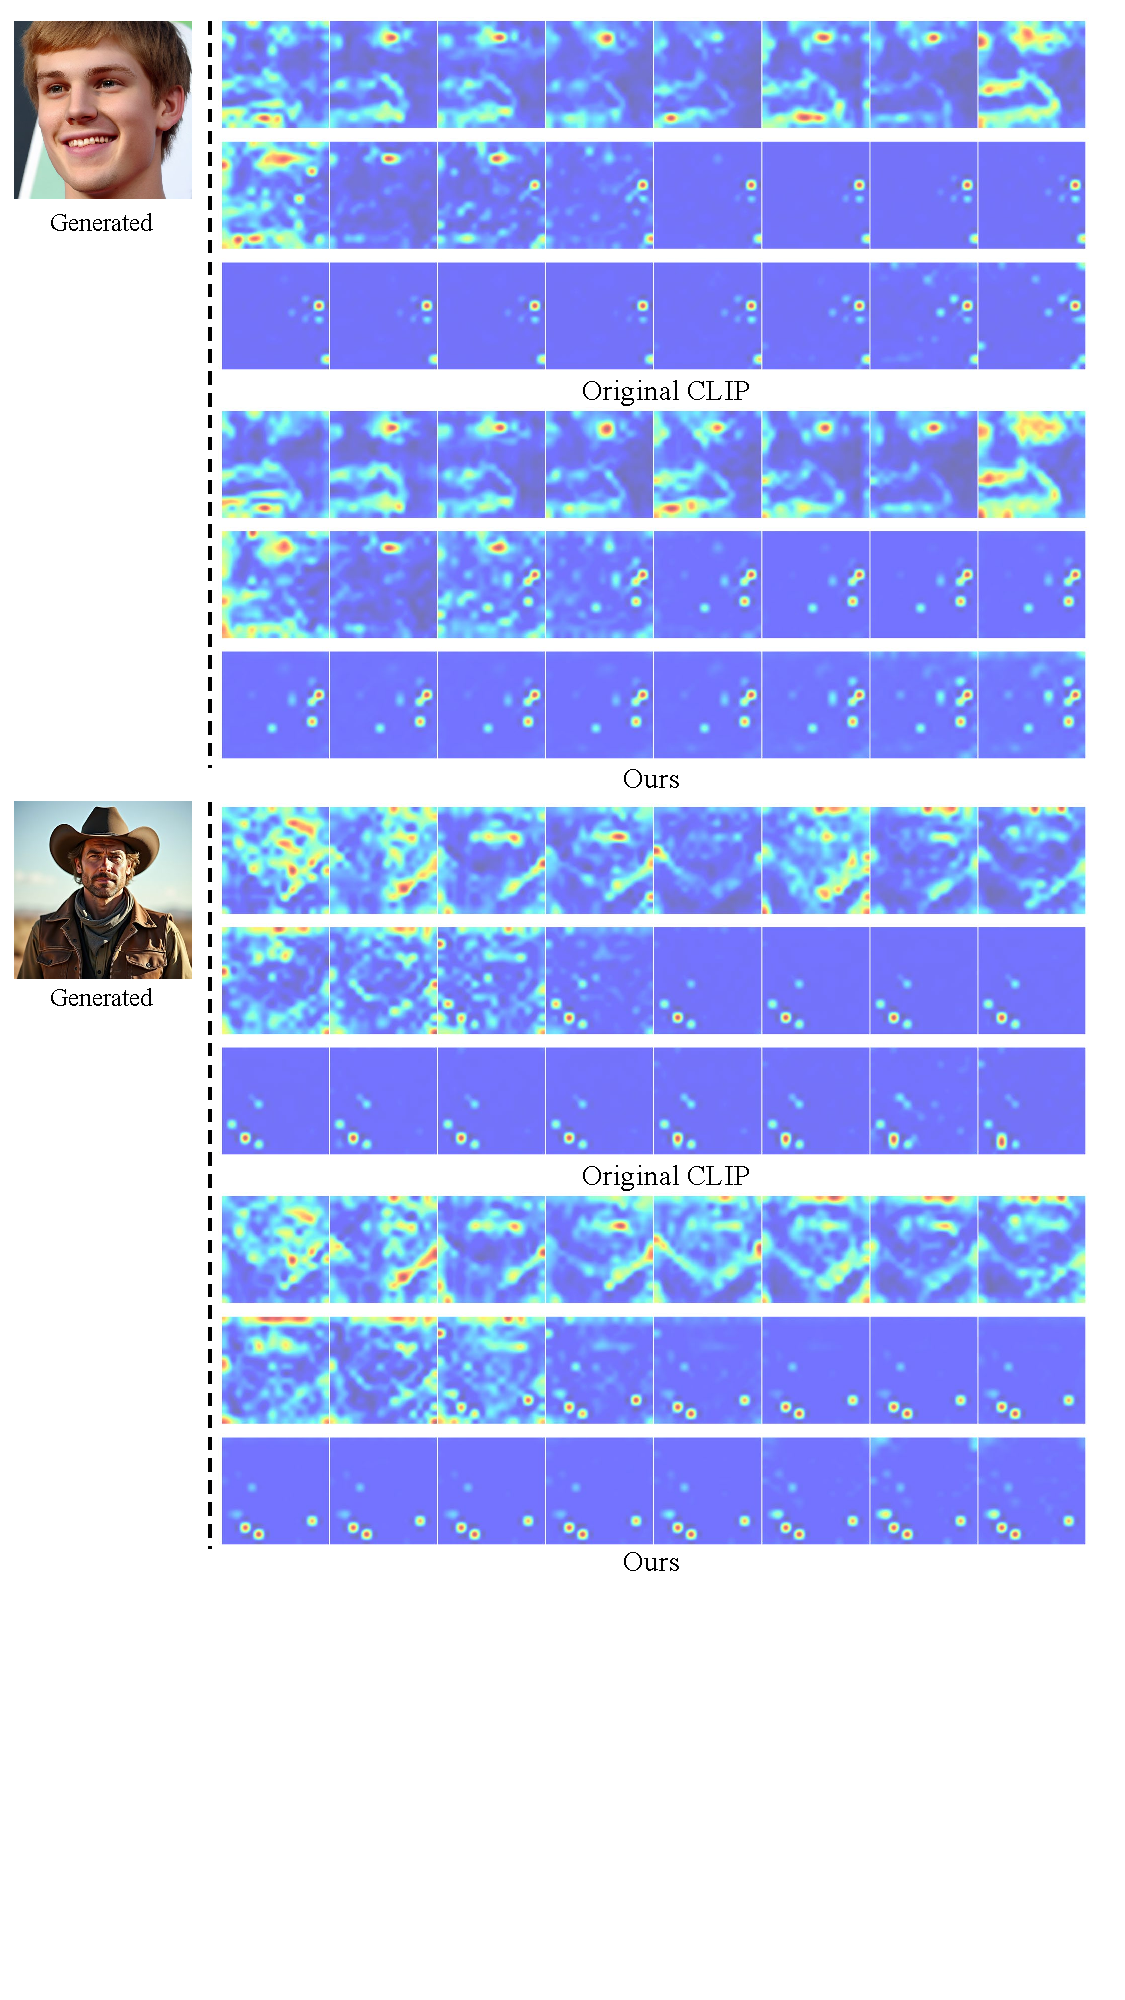
\includegraphics[width=0.85\linewidth]{figs/attentionmap1.pdf} 
        \caption{\textbf{Self-Attention map} between original CLIP backbone and our finetuned backbone. There are 24 ViT blocks in the image encoder, we plot 8 blocks in each row, with indices increasing from left to right. For clarity of visualization, we use bicubic interpolation between image patches. In the shallow layers, we preserve most semantic features, in deep layers, our attention includes a wider range compared to original CLIP. }
        \label{fig:attention1} 
\end{figure*}

\begin{figure*}[!t]
        \centering
        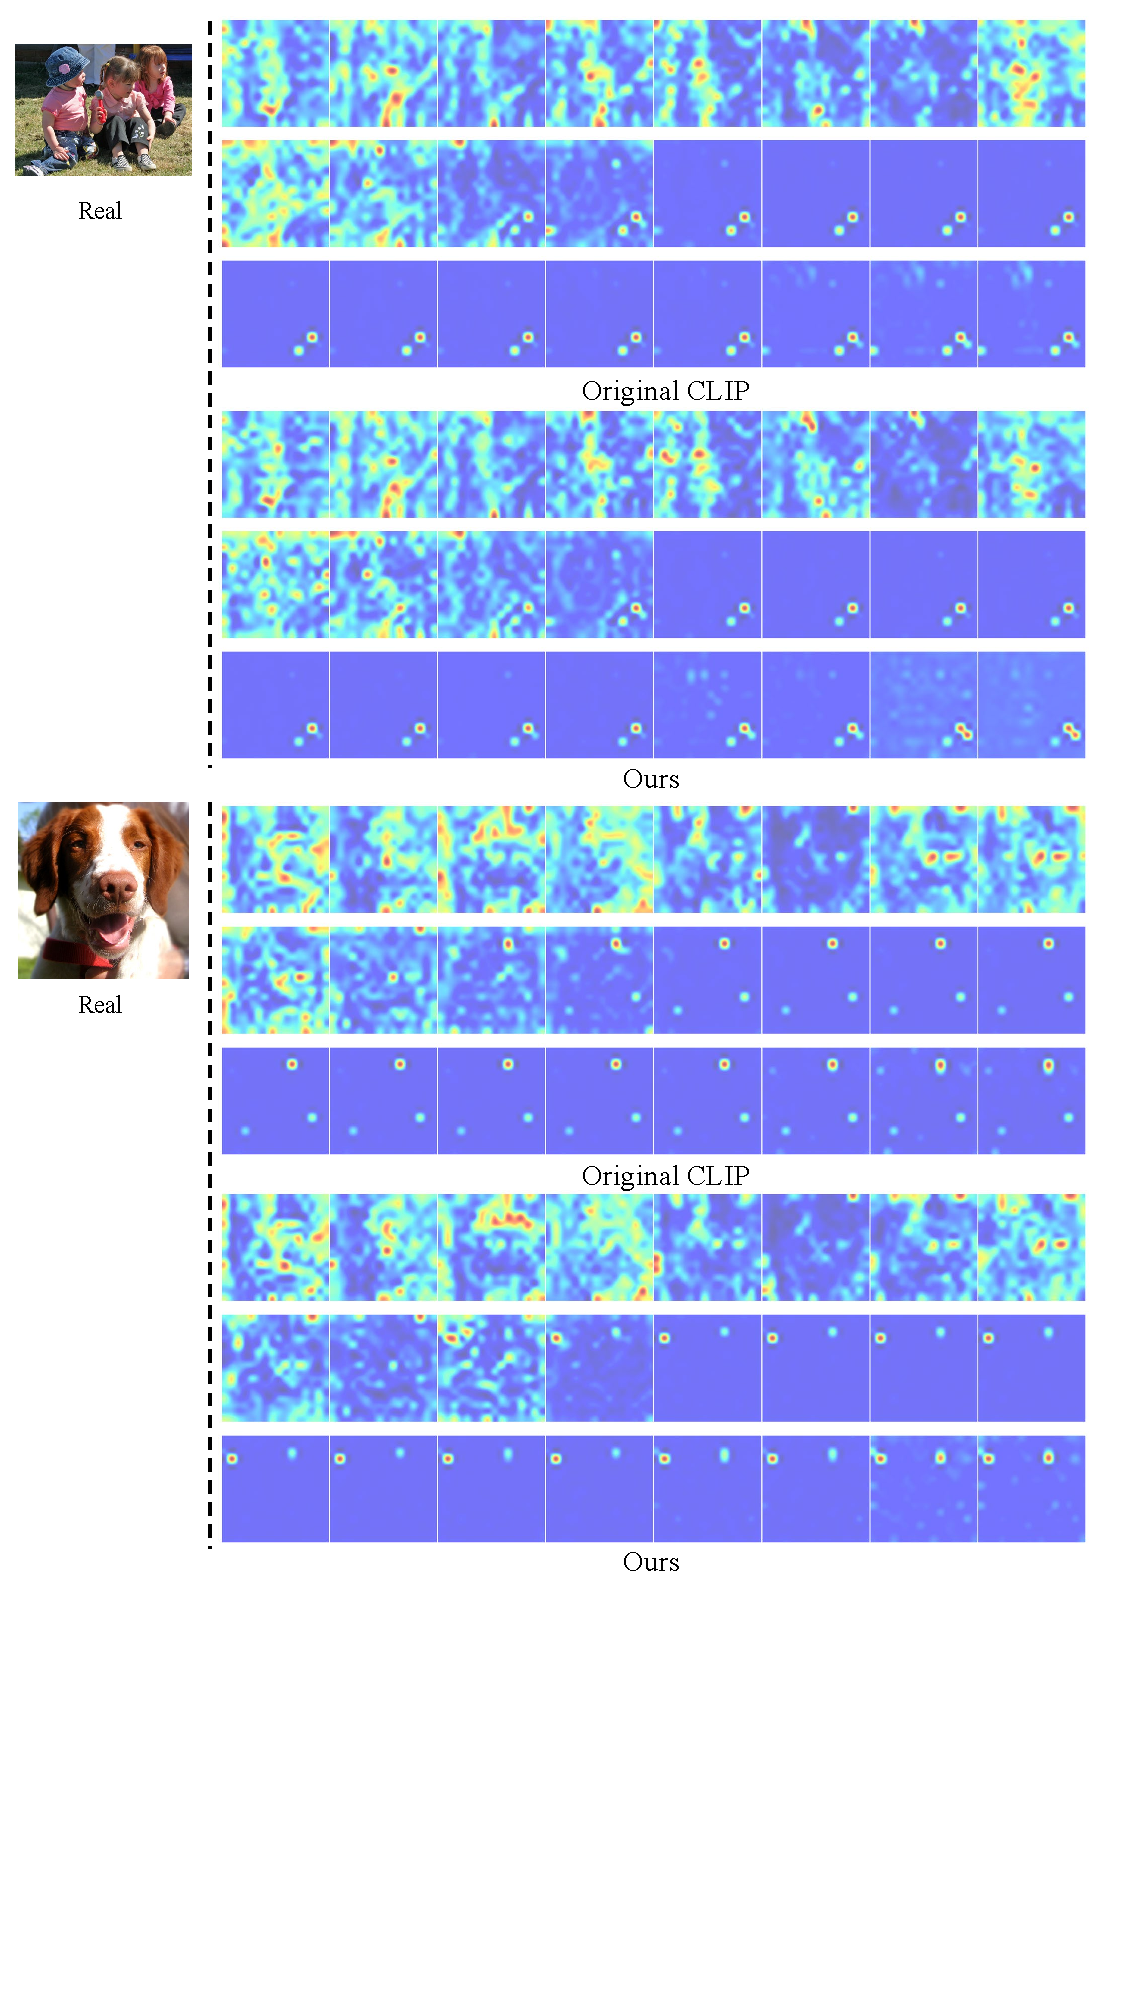
\includegraphics[width=0.85\linewidth]{figs/attentionmap2.pdf} 
        \caption{\textbf{Self-Attention map} between original CLIP backbone and our finetuned backbone. There are 24 ViT blocks in the image encoder, we plot 8 blocks in each row, with indices increasing from left to right. For clarity of visualization, we use bicubic interpolation between image patches. In the shallow layers, we preserve most semantic features, in deep layers, our attention includes a wider range compared to original CLIP.}
        \label{fig:attention2} 
\end{figure*}

\clearpage      % <<< 把前面所有未排版完的浮动体全部排完，再开始参考文献
{
    \small
    \bibliographystyle{ieeenat_fullname}
    \bibliography{main}
}

% WARNING: do not forget to delete the supplementary pages from your submission 

\end{document}
